\section{Design Criteria}

Our pertinent criteria for alloys with the potential to supercede nickel-base superalloys have been drawn up using a representative 2$^{nd}$ generation nickel superalloy, CMSX--4, as a benchmark. We want creep and tensile properties to be an additional 100\celsius above CMSX--4. The material's density has to be less than 9.0 \gram\usk\centi\rpcubic\metre. Oxidation resistance needs to be an innate property, and an adherent thermodynamically stable, slow-growing oxide layer that has low oxygen permeability is required.  The three oxides that meet these criteria are those of chromium, aluminium and silicon (Figure \ref{fig:IntermetallicOxidation}).
%
\begin{figure}[H]
\begin{center}
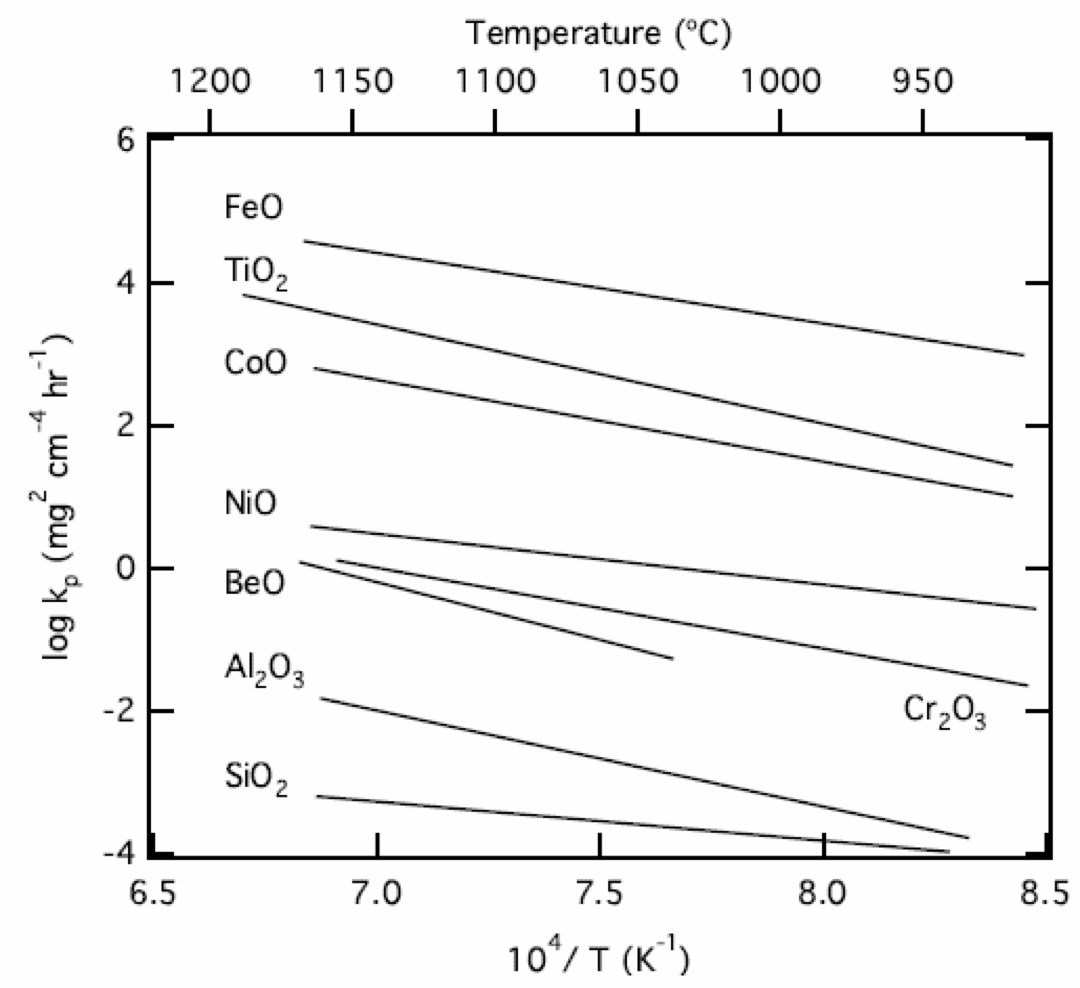
\includegraphics{IntermetallicOxidation}
\caption{Parabolic growth constants of oxides on select ordered intermetallics.}\label{fig:IntermetallicOxidation}
\end{center}
\end{figure}
%
For alloys used at low to intermediate temperatures, chromium oxide is the preferred oxide as it has excellent corrosion resistance at this range of temperatures. Once placed in an environment with temperatures of higher than 1000\celsius, chromium oxide becomes thermodynamically unstable and volatilises. Thus, such alloys are inappropriate for use at high temperatures. Historically, alumina has been the oxide of choice for high temperature materials; however, aluminium-based intermetallics display mediocre high temperature mechanical properties. As for silicon-containing materials studies indicate that several systems possess good high temperature creep properties, but many systems still remain relatively unexplored. Silicon-containing systems will be explored to establish potential candidate systems to incorporate in our alloy design. 	

\section{A--A$_3$Si Alloy Design}
\subsection{Key Issues to Address}
Investigations of silicide-based high temperature alloys have focused on achieving creep resistant alloys at higher temperature capabilities than those of nickel-base superalloys. The low fracture toughnesses of 2--5 \mega\pascal\usk\meter$^{\frac{1}{2}}$ of monolithic intermetallics at room temperature, which is a fraction of a K$_{IC}$ of 15 \mega\pascal\usk\meter$^{\frac{1}{2}}$, the value that is generally agreed upon that is required for an alloy to be machinable ~\cite{raj95}. Due to the bonding nature of intermetallics and the existence of low energy cleavage planes, it will be difficult to improve fracture toughnesses substantially.

One approach to resolve this issue would be to introduce a toughening phase into the alloy.  For effective toughening, a continuous phase would be desirable ~\cite{kahn80}. By doing so, the load bearing area would effectively be reduced, and alloys of such a system would have lower creep resistances than intermetallic-intermetallic systems at a given temperature. Many intermetallic systems that are currently under investigation possess poor oxidative properties ~\cite{harris97}. One such system is the molybdenum - silicon binary.  Although all phases in this binary are susceptible to catastrophic oxidation at intermediate temperatures, their high temperature mechanical properties are being extensively researched. We do desire materials with higher temperature capability, but not at the expense of intermediate temperature properties. A turbine blade in an aero-engine's hot section experiences temperatures from 650\celsius\ at the blade base to 1100\celsius\ at the blade tip. Investigation of intermetallics in this system with higher silicon contents, such as MoSi$_2$, was undertaken in an attempt to increase the propensity for silica scale formation.  This compromised mechanical properties ~\cite{rawn01} and did not suppress pesting ~\cite{yanagihara96}. 

Tertiary elements such as Al were added on the basis that they had larger affinities to oxygen than Si and would be able to form a protective oxide layer.  However, Al has been added solely for its oxidative properties; extensive research on Al-based intermetallics have shown that they do not have good high temperature creep properties. This method is not ideal, as it compromises mechanical properties in order to improve oxidative properties, but fails to address other issues, such as the inherent low fracture toughness of such systems. 

The fact that arc-melted silicides with micro-cracks out-perform powder-processed ingots shows that the creep properties reported thus far are not an accurate reflection of the true potential of silicides.  This can be resolved provided production techniques can be developed. Designing alloys based on eutectic systems would lower the required casting temperature appreciably, and increase the likelihood of castability.  Low coeffficient of thermal expansion (CTE) anisotropy and high thermal conductivity can help minimise the extent of micro-crack formation during solidification.


\subsection{Silicide Selection}

To achieve effective damage tolerance, a toughening phase occurring as a continuous matrix is preferred over discrete particles.  By focusing our design efforts around eutectic systems that contain a solid solution phase, we seek to address two main issues.
\begin{enumerate}
\item Alloy microstructure can be designed with a continuous solid solution matrix.  \item Eutectics have substantially lower melting temperatures than the constituent intermetallics.
\end{enumerate}  
  This can allow increased ease of material manufacture and microstructural optimisation if the casting temperatures are lower than the maximum temperatures attain by existing or emerging equipment. There are only 10 A--A$_x$Si$_y$ silicide systems that contain a solid solution toughening phase and an intermetallic load-bearing phase, with a density of less than 9.0 \gram\usk\centi\rpcubic\metre. They must also have a high eutectic temperature that is higher than 1500\celsius, and have no phase transformation between room temperature and an operating temperature of 1200\celsius.  This reduces the number of candidates to Cr--Cr$_3$Si, Hf--HfSi$_2$, Mo--Mo$_3$Si, V--V$_3$Si and Y--Y$_5$Si$_3$, where the Cr, Mo and V systems have the same chemical formula A--A$_3$Si. The crystal structure of these two phases are shown in Figures \ref{fig:BCC} and \ref{fig:A15}. Basing the alloy design around the above three transition metal silicide systems is beneficial (Figure \ref{fig:periodictable}). 
%
\begin{enumerate}
\item Cr and V have low densities.
\item The A15 phase is cubic, which a simple crystal structure for an intermetallic.
\begin{enumerate}
\item it is more likely to possess sufficient equivalent independent slip systems.
\item it is more likely to permit plastic deformation at lower temperatures.
\end{enumerate}
\item Extensive alloying is possible because the formation of undesirable phases during will be minimised.
\begin{enumerate}
\item Cr and V are perfectly miscible.
\item Mo and V are perfectly miscible.
\item Cr$_3$Si and V$_3$Si are perfectly miscible.
\item Mo$_3$Si and V$_3$Si are perfectly miscible.
\end{enumerate}
\item All three systems have non-faceted/ non-faceted behaviour.
\begin{enumerate}
\item They form lamellar microstructures when solidified.
\item This increases fracture toughness.
\end{enumerate}
\end{enumerate}    
%
\begin{figure}[H]
\begin{center}
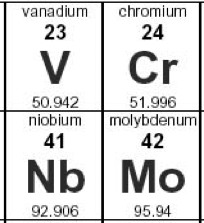
\includegraphics[width=4cm]{periodictable}
\caption{Portion of the periodic table showing the relative positions of Cr, Mo, Nb and V.}
\label{fig:periodictable}
\end{center}
\end{figure}
%
As mentioned, these systems have non-faceted/ non-faceted behaviour and form lamellar microstructures when solidified (Figures \ref{fig:growthmorphologies} and \ref{fig:DS_Cr-Cr3Si}) ~\cite{bei03}. The directionality of the lamellae can be controlled by directional solidification.  Slow solidification rates allow a planar growth front to be maintain, which allows for a neat lamellar structure to form. With fast solidification rates, the planar growth front breaks down, resulting in a cellular structure instead (Figure \ref{fig:DS_Cr-Cr3Si_bad}). The other scenario, non-faceted/faceted, is exemplified by nickel-base superalloys. They experience dendritic growth during fast solidification.
%
\vspace{1cm}
\begin{figure}[H]
\begin{center}
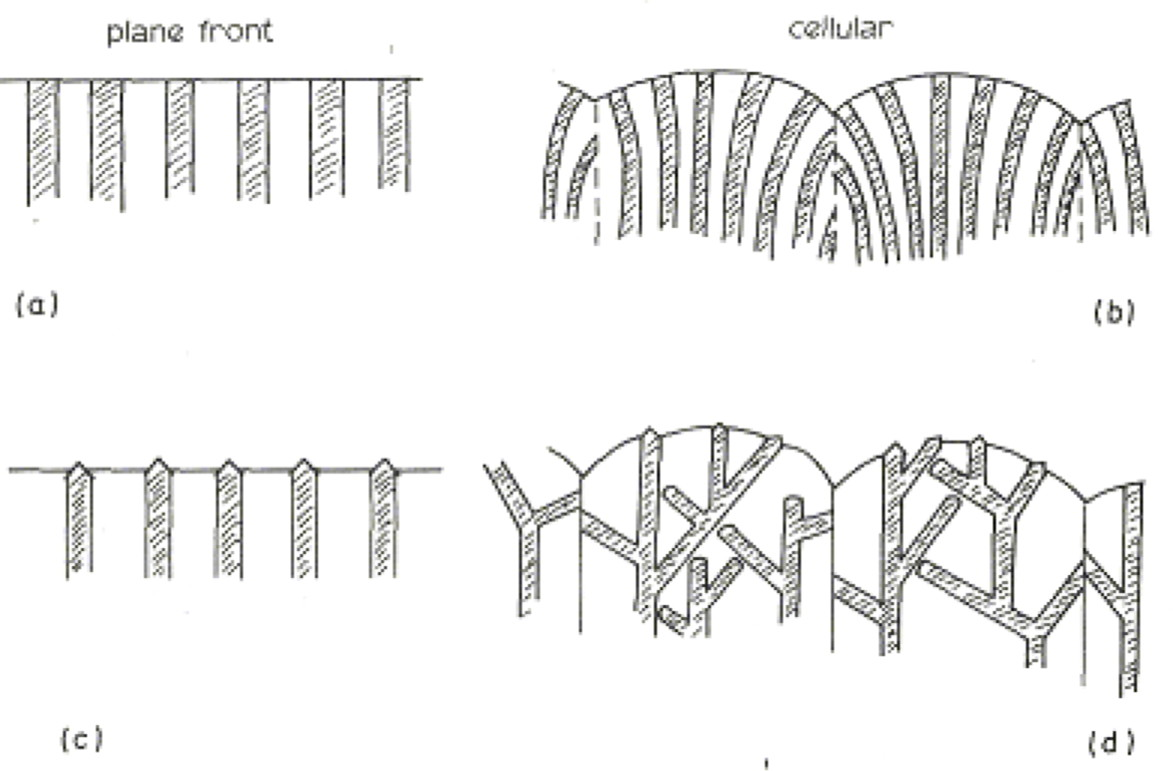
\includegraphics[width=.6\textwidth]{growthmorphologies}
\caption{Eutectic Growth Morphologies formed by planar and non-planar growth fronts.}\label{fig:growthmorphologies}
\end{center}
\end{figure}
%

\begin{figure}[hp!]
\begin{center}
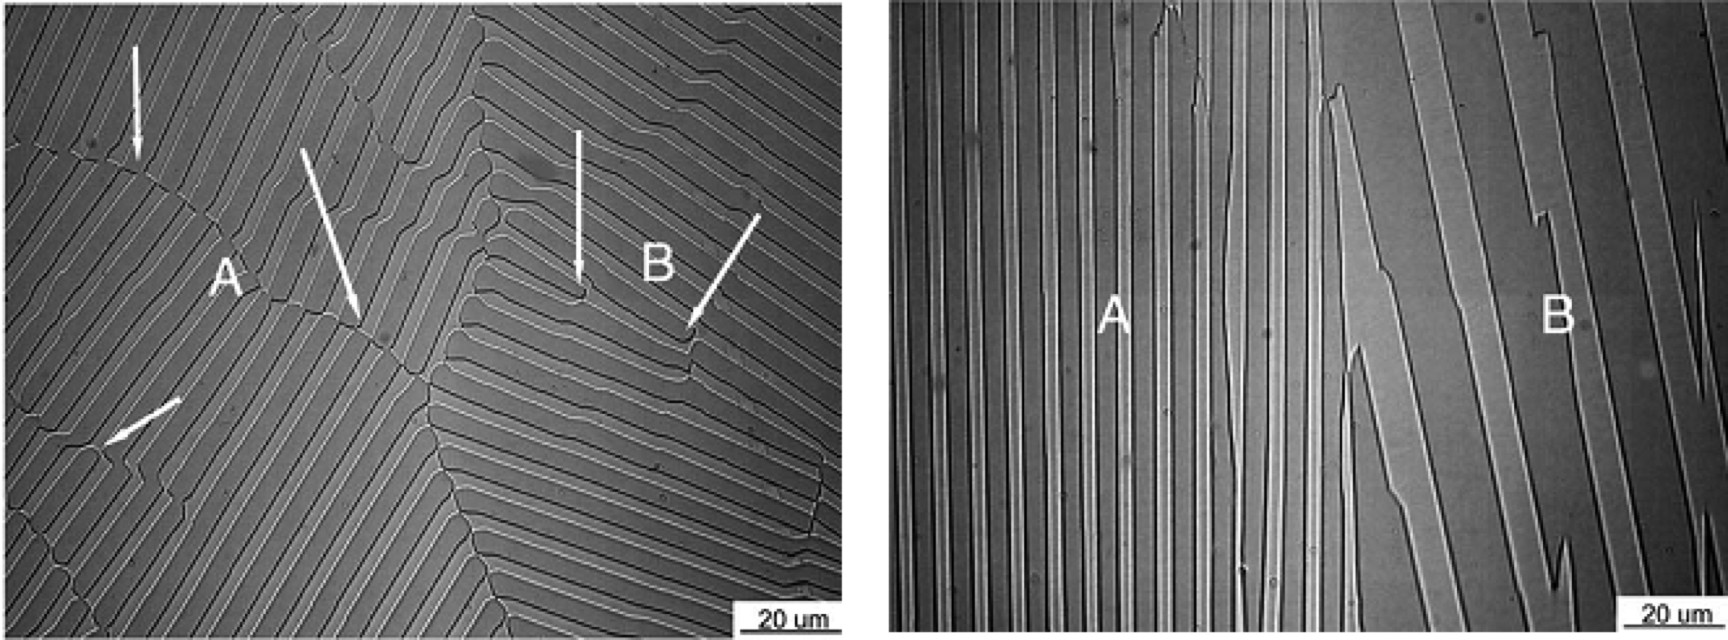
\includegraphics[width=\textwidth]{DS_Cr-Cr3Si}
\caption{Cr-Cr$_3$Si eutectic alloy directionally solidified at 40 mm/h and 60 rpm: (a) transverse and (b) longitudinal sections ~\cite{bei03}.}\label{fig:DS_Cr-Cr3Si}
\end{center}
\end{figure}
%
\begin{figure}[hp!]
\begin{center}
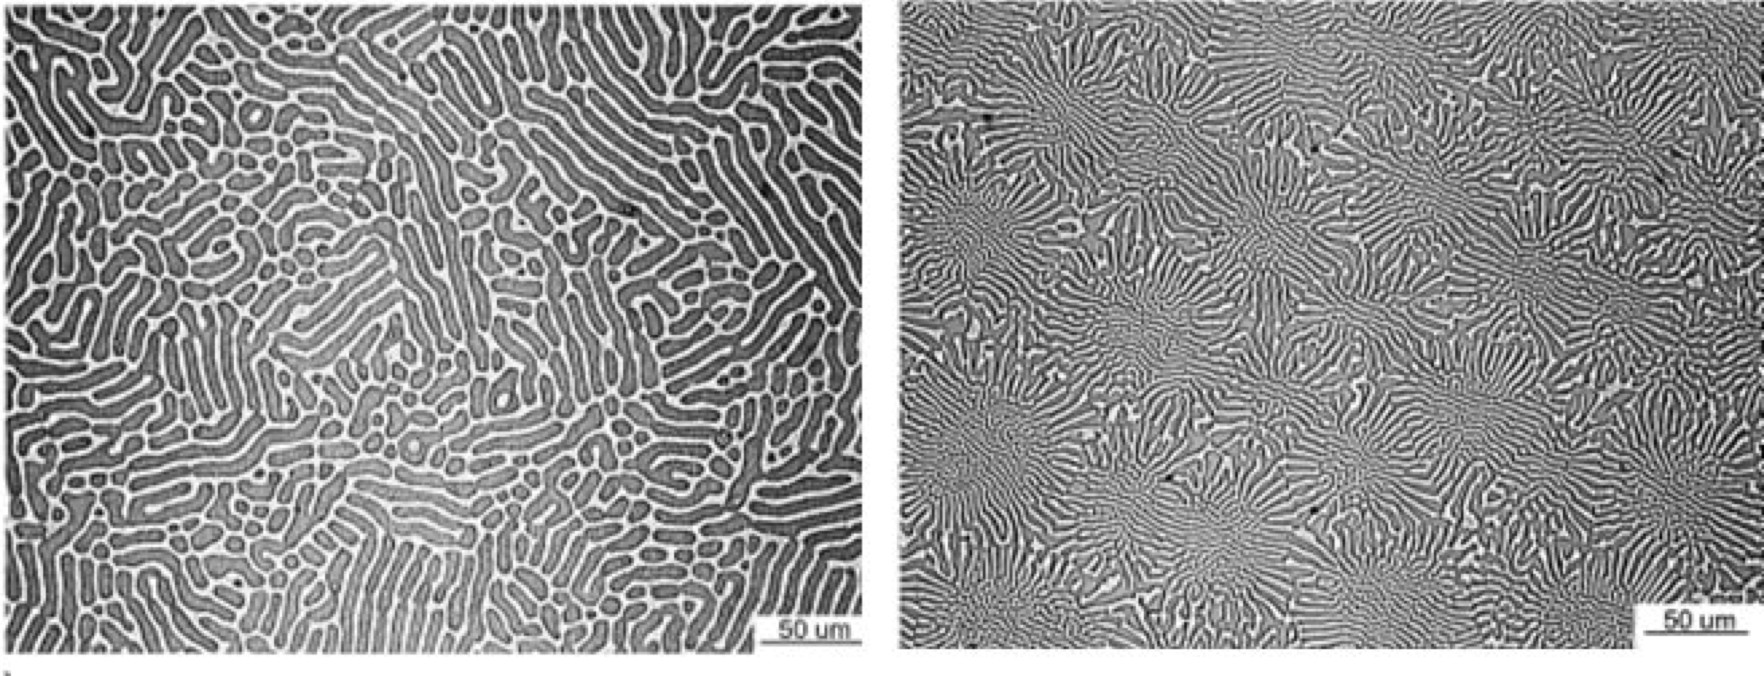
\includegraphics[width=\textwidth]{DS_Cr-Cr3Si_bad}
\caption{Cr-Cr$_3$Si eutectic alloy directionally solidified at 150 mm/h and 60 rpm, transverse section, displaying cellular structure ~\cite{bei03}. }\label{fig:DS_Cr-Cr3Si_bad}
\end{center}
\end{figure} 
%
\begin{figure}[H]
\begin{center}
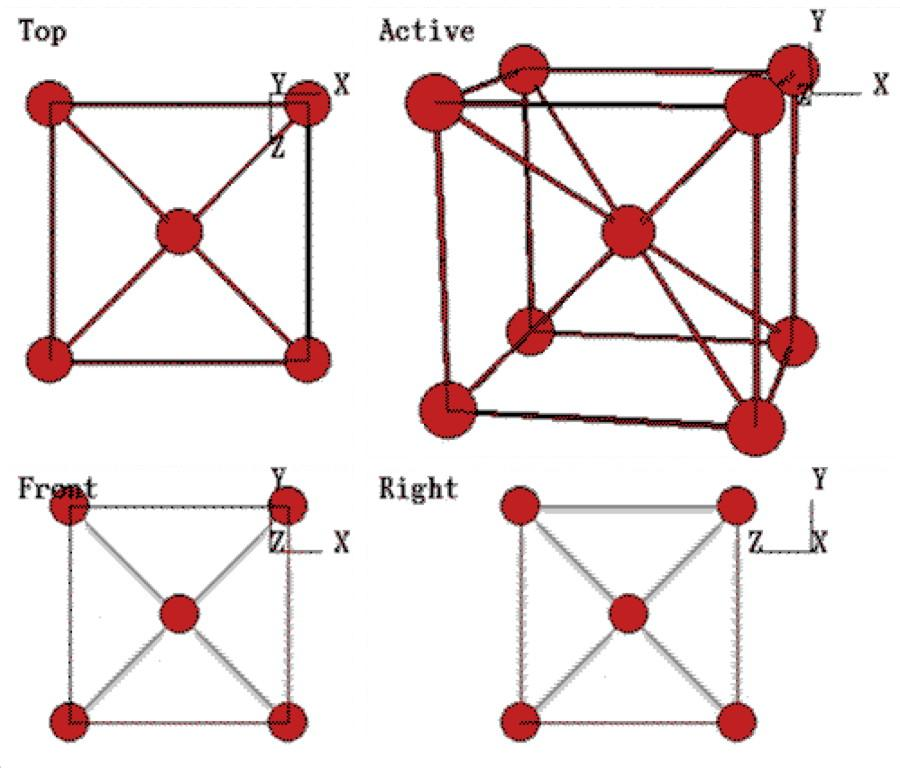
\includegraphics[width=9cm]{BCC}
\caption{The body centered cubic structure of the solid solution ~\cite{ashcroft76}.}\label{fig:BCC}
\end{center}
\end{figure} 
%
\begin{figure}[H]
\begin{center}
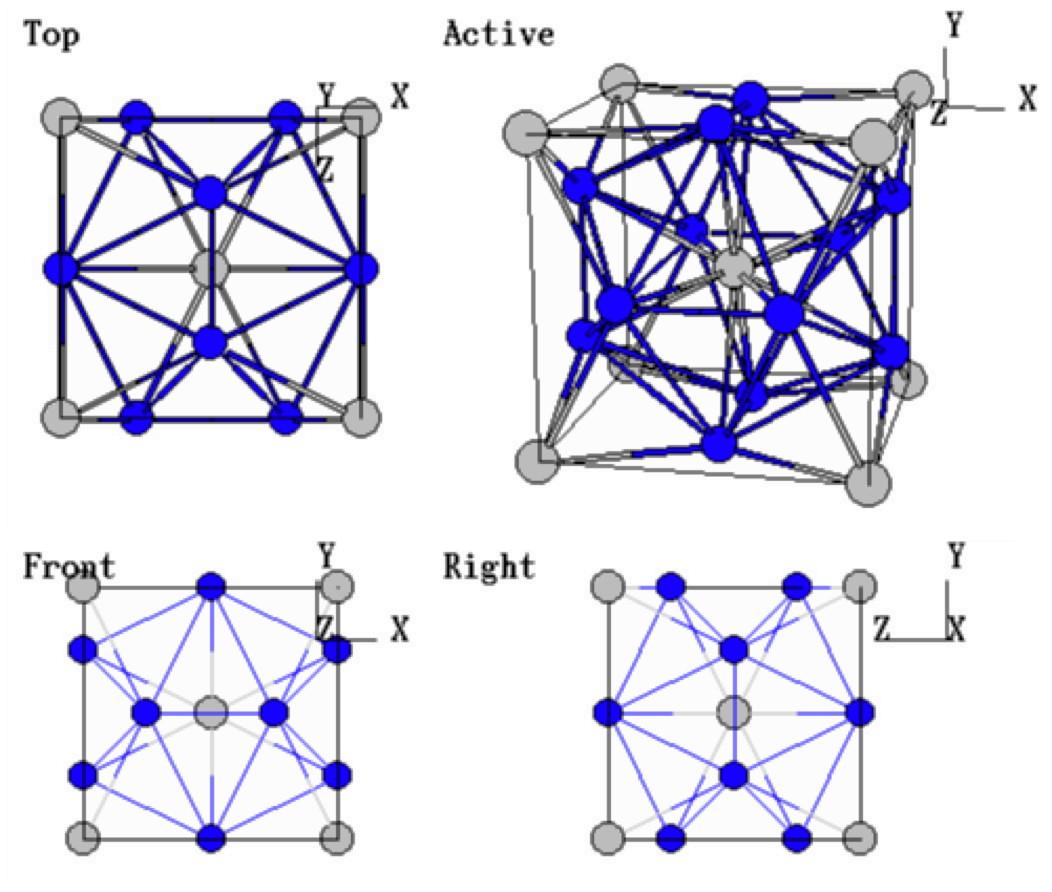
\includegraphics[width=9cm]{A15}
\caption{The A15 structure of A$_3$Si ~\cite{nevitt95}.}\label{fig:A15}
\end{center}
\end{figure}
Preliminary results show silicides with unoptimised microstructures containing micro-cracks display creep properties with a 200\celsius\ increase in temperature capability over nickel-base superalloys (Figures \ref{fig:creepshah92_1} and \ref{fig:creepshah92_2}.  However, these silicides have not been designed to contain a toughening phase and are very brittle, possessing poor fracture toughness at room temperature. 
%
\begin{figure}[H]
\begin{center}
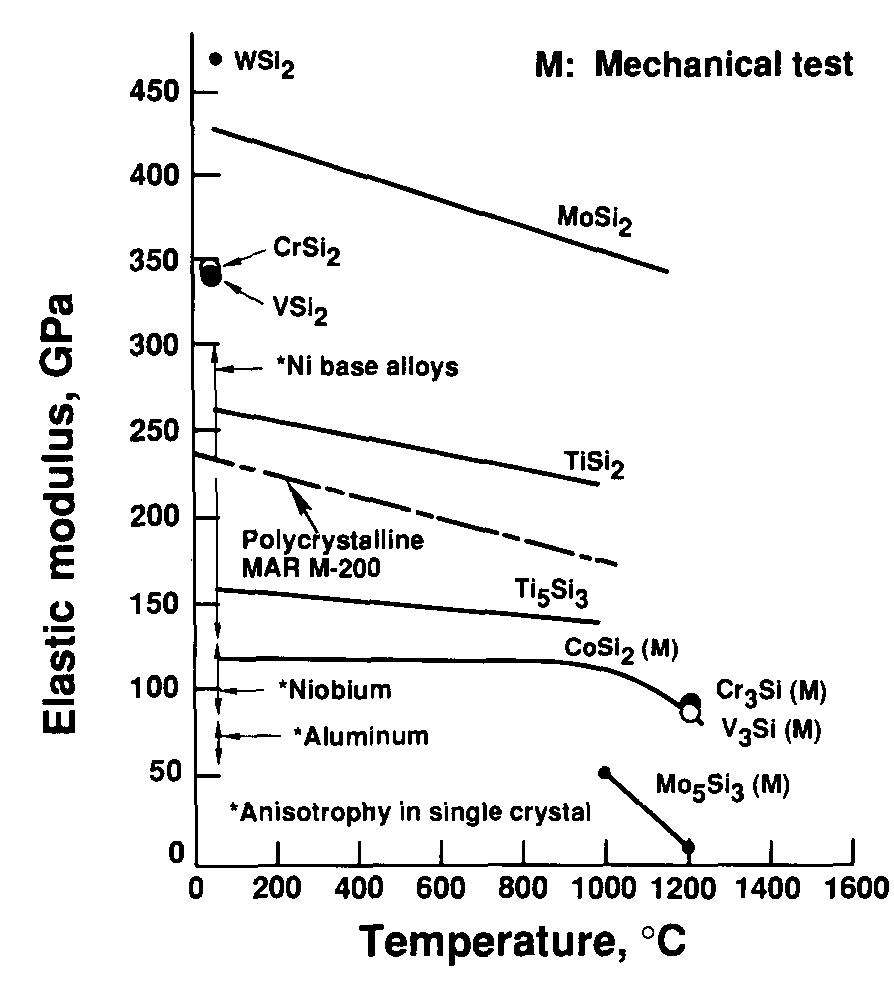
\includegraphics[width=.6\textwidth]{creepshah92_1}
\vspace{-.3cm}
\caption{Compressive creep properties of candidate systems and nickel-base superalloys ~\cite{shah92}.}\label{fig:creepshah92_1}
\end{center}
\end{figure}
\vspace{-.5cm}
%
\begin{figure}[H]
\begin{center}
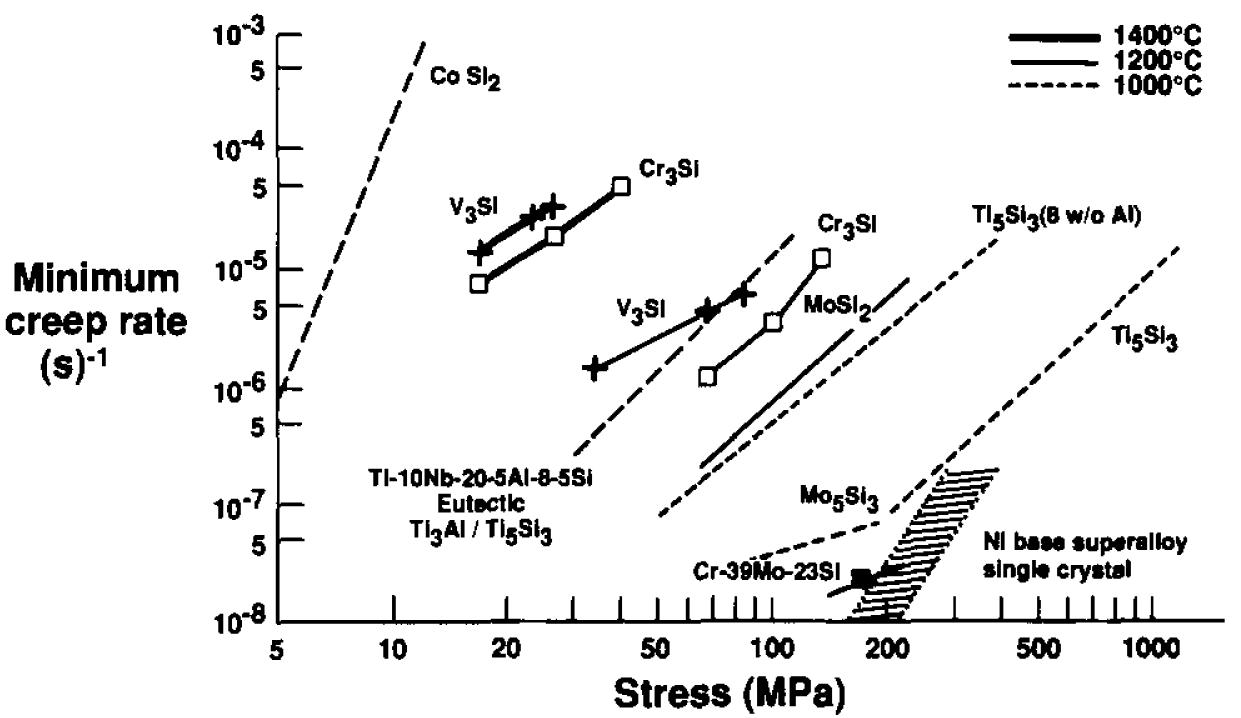
\includegraphics[width=.9\textwidth]{creepshah92_2}
\caption{Comparison of minimum compressive creep rate of silicides and nickel superalloys vs stress between 1000-1400\celsius\ ~\cite{shah92}.}\label{fig:creepshah92_2}
\end{center}
\end{figure}
%
\subsection{A--A$_3$Si Eutectics}

The first system to be assessed would be the Cr--Cr$_3$Si eutectic.  This eutectic system can help to counter the occurrence of ``pesting" as the character of chromium oxide is excellent for oxidation and corrosion resistances up to 1000\celsius ~\cite{raj95a}.  It is extensively used in alloy systems such as steel and nickel-base superalloys ~cite{reed06}. Cr is known to be a solid solution that is prone to nitrogen embrittlement and notch sensitivity ~\cite{abrahamson57}.  It is very sensitive to impurity content and its ductile-brittle transition temperature (DBTT) can range from 50--500\celsius\ (Figure \ref{fig:Cr_ductility}).  This can be most effectively brought down to 40\celsius\ through extensive alloying with ruthenium ~\cite{abrahamson57}.  This DBTT is not ideal as it is not below room temperature, and such additions would increase material costs and alloy density.
%
\begin{figure}[H]
\begin{center}
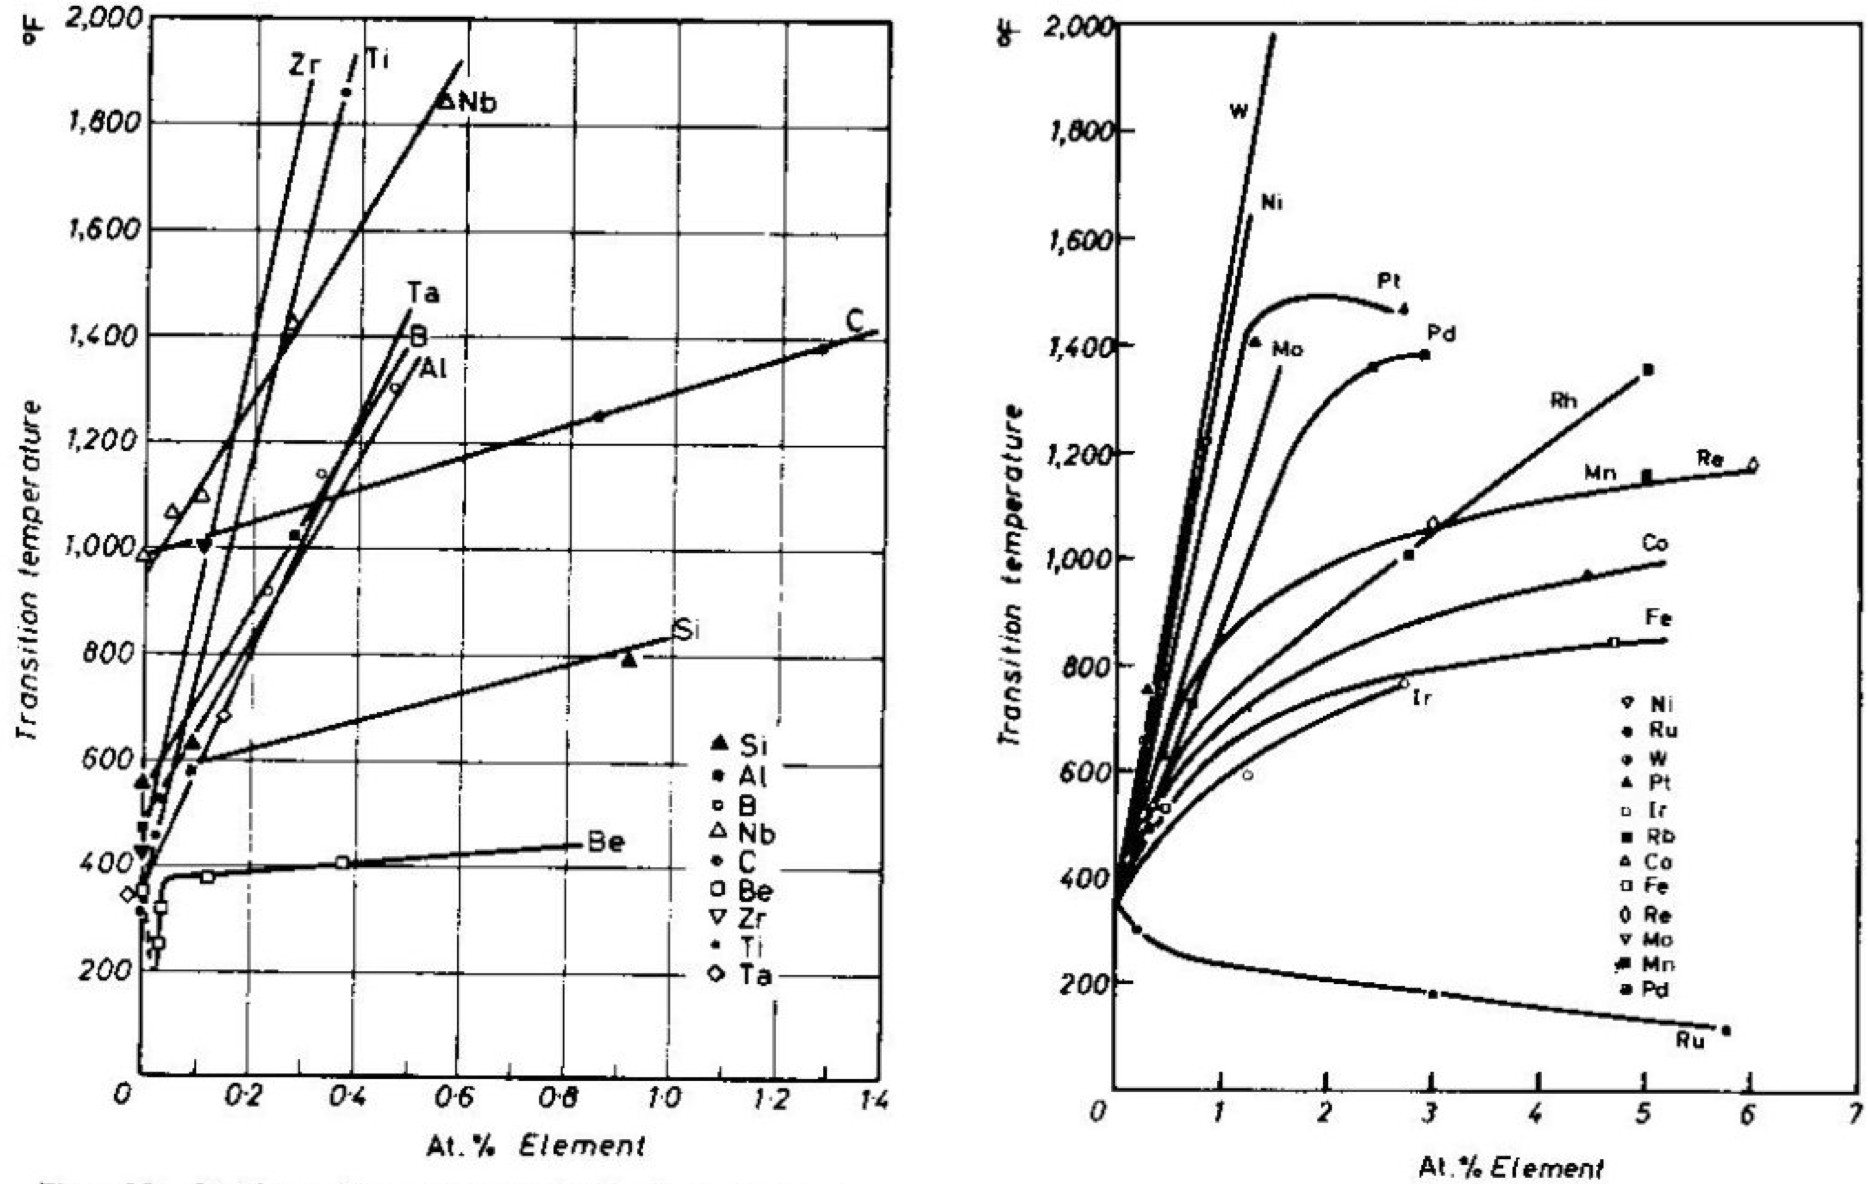
\includegraphics[width=.98\textwidth]{Cr_ductility}
\vspace{-2mm}
\caption{Initial transition temperature for 65$^\circ$ bend versus at.\% alloying addition ~\cite{abrahamson57}. }\label{fig:Cr_ductility}
\end{center}
\end{figure}
\vspace{-8mm}
%
Cr--Cr$_3$Si has the lowest melting point out of the 3 systems at 1705\celsius\ ~\cite{gokhale90}. The elastic constants of Cr$_3$Si have been reported by Bei et al.  to be between 98--412 GPa ~\cite{bei04}. Another system that will be looked at is the V--V$_3$Si eutectic.  Vanadium is tough; DBTT values between -110 and -65\celsius\ have been reported ~\cite{dunn61}. Data on the effect that vanadium has on the DBTT of chromium has not been found, but alloying vanadium with chromium can result in a solid solution with good room temperature fracture toughness. The creep performance of V$_3$Si is better than Cr$_3$Si at 1400\celsius\ (Figure \ref{fig:creepshah92_2}), and it retains its hot hardness better than Cr$_3$Si (Figure \ref{fig:VCr_hardness}). It is over twice as hard as Cr$_3$Si at 1100\celsius.  
%
\begin{figure}[H]
\begin{center}
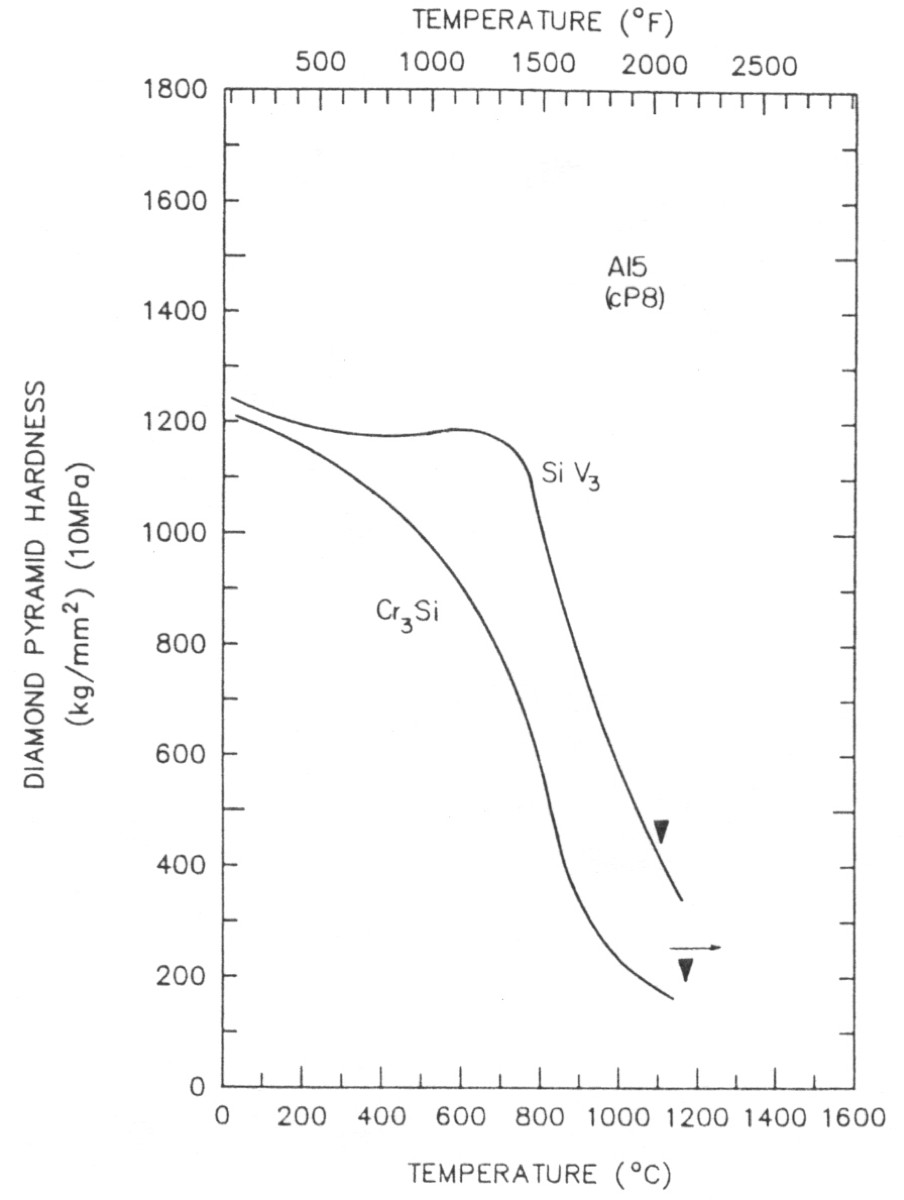
\includegraphics[width=7cm]{VCr3Si_hardness}
\vspace{-2mm}
\caption{Hardness of Cr$_3$Si and V$_3$Si as a function of temperature.}\label{fig:VCr_hardness}
\end{center}
\end{figure}
\vspace{-1cm}
%
Chromium and vanadium form a perfectly miscible body-centered cubic solid solution (Figure: \ref{fig:CrV}) ~\cite{kocherzhinskii85}, and alloying can decrease the number of ordered bonds to increase toughness. The two intermetallics Cr$_3$Si and V$_3$Si are perfectly miscible as well (Figure: \ref{fig:Cr3Si_alloying}) ~\cite{shah92}. The phase diagram of Cr--V--Si is unavailable. This suggests that no additional phases will form if one were to move across the tie-line from eutectic Cr--Cr$_3$Si towards V--V$_3$Si, as Cr and V can completely substitute for each other. As there are no ternary phase diagrams available for the Cr--V--Si system, the location of the eutectic trough in ternary space will need to be determined.
%
\vspace{1mm}
\begin{figure}[H]
\begin{center}
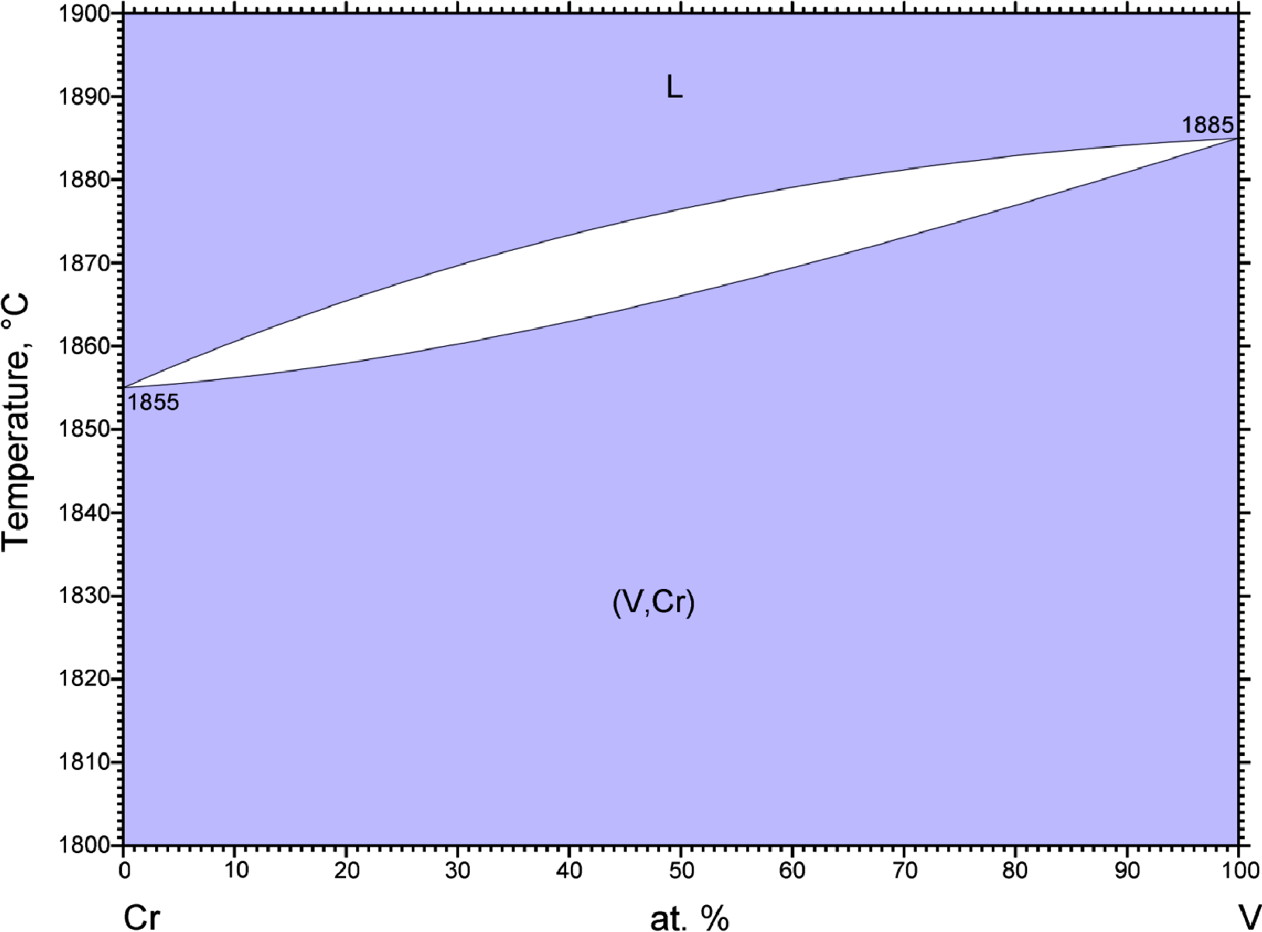
\includegraphics[width=9cm]{CrV}
\caption{Binary phase diagram of Cr and V ~\cite{kocherzhinskii85}.}\label{fig:CrV}
\end{center}
\end{figure}
%
\begin{figure}[H]
\begin{center}
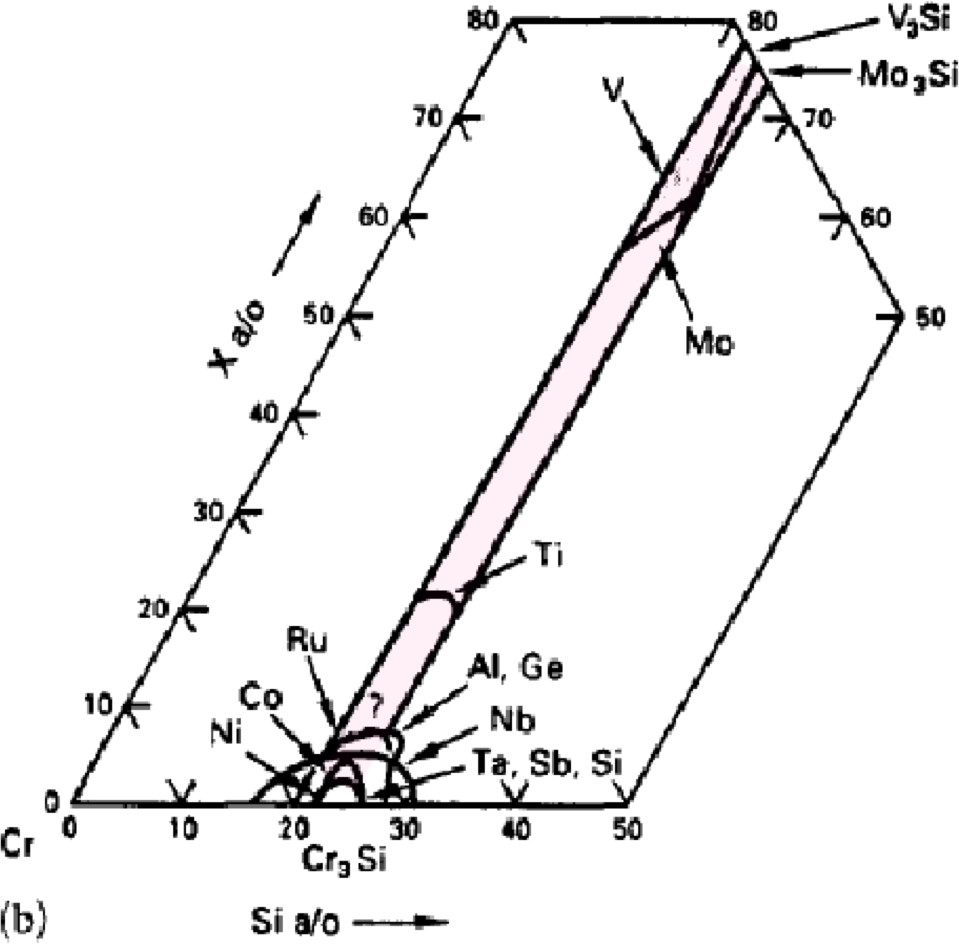
\includegraphics{Cr3Si_alloying}
\caption{Effect of Ternary additions to the Cr$_3$Si phase field ~\cite{shah92}.}\label{fig:Cr3Si_alloying}
\end{center}
\end{figure}
\vspace{-5mm}
%
As oxidation resistance needs to be an inherent property of a turbine blade material, a preliminary study of the oxidation behaviour of these tie-line eutectics needs to be conducted to determine which, if any, eutectic compositions has sufficient oxidation resistance. An alloy with sufficient oxidation resistance needs to form an adherent Cr$_2$O$_3$ layer at low and intermediate temperatures, and an adherent SiO$_2$ layer at high temperatures. This would probably result in a dual-layer oxide structure. It is suspected that substituting vanadium for chromium can result in a more oxidation resistant alloy, as all vanadium oxides volatise between 600--1200\celsius\ ~\cite{wriedt90}. During oxidation, and oxides of vanadium will undergo sacrificial oxidation and will not compete with Cr$_2$O3 and SiO$_2$ to form oxide layers. SiO$_2$ has the lowest parabolic rate constant out of Al$_2$O$_3$, Cr$_2$O3 and SiO$_2$, and decreasing chromium concentration can help prevent the oxidation of silicon from being overwhelmed by that of chromium during the onset of oxidation. SiO$_2$ could thereby have a better chance of forming a continuous layer. This can help combat the poor high temperature oxidation resistance of Cr$_3$Si reported by Raj ~\cite{raj95}. In the event that vanadium does not preferentially oxidise initially, a layer of vanadium-rich material will form just beneath the oxide layer. Upon oxide spallation, runaway may occur, as vanadium oxides are volatile and not protective. 

Shah reports that single crystal material is less likely to pest than material with uncontrolled coarse grain structure ~\cite{shah92}. He also states that single-crystal cubic intermetallics with isotropic CTE and low DBTT are not likely to pest, referring to his preliminary observations on Cr$_3$Si and CoSi$_2$. The pest effect was not investigated in the V-Si binary. Investigating the oxidation behaviour at intermediate and high temperatures of the eutectic compositions between Cr--Cr$_3$Si and V--V$_3$Si can verify if pesting is an issue.

%

\begin{figure}[H]
\begin{center}
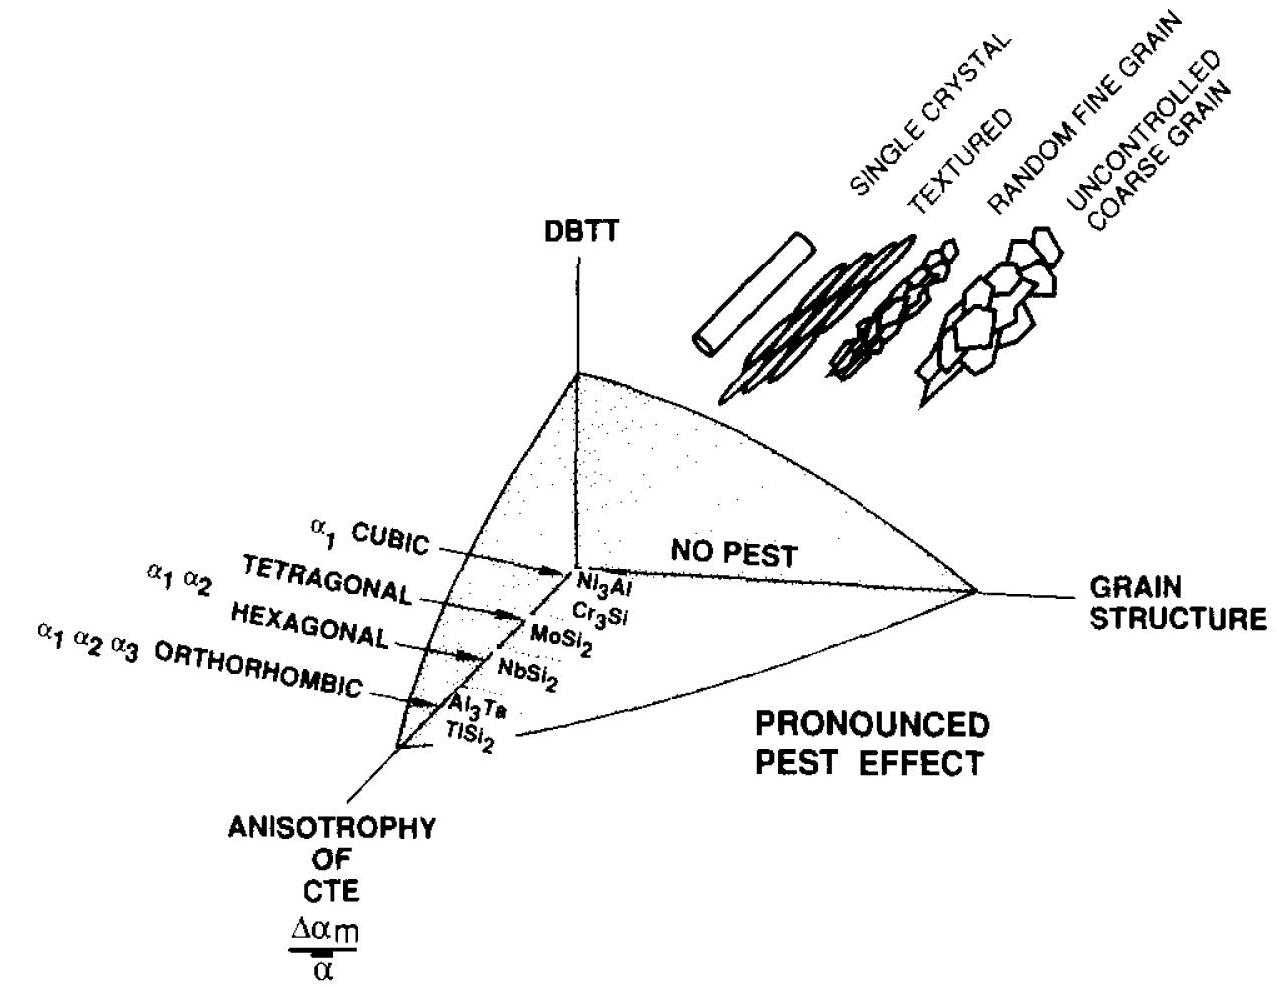
\includegraphics[width=.78\textwidth]{shahpest}
\caption{Schematic map showing the effect of the DBTT, the nature of the grain structure and the anisotropy of the CTE on the pest effect ~\cite{shah92}.}
\label{fig:shahpest}
\end{center}
\end{figure}
\vspace{-9mm}
%
The temperature dependence of the alloys' specific weight change for a given exposure time may be presented as a way of ranking oxidation resistance. This will help clarify the effects of a Cr$_2$O$_3$ and SiO$_2$ dual-layer structure on oxidation properties. Due to the novel and intricate alloy manufacturing required, we need to determine whether we are able to reproduce the lamellar and cellular microstructures of Bei et al.. If successful, we will attempt to manufacture material of the same microstructure for the V--V$_3$Si eutectic. 

The effect lamellar spacing has on an alloy's high temperature mechanical properties will then be studied. It is suspected that cellular microstructures may exhibit better mechanical properties. With a smaller lamellar spacing, it will be more effective at crack deflection, and may even possess a spacing that is smaller than the critical crack length of the material, effectively toughening it through crack containment. Also, they are more anisotropic, and can better sustain impacts in the transverse direction. 

Several groups have reported that Mo substitutions for Cr in monolithic Cr$_3$Si result in improvements in both high temperature creep capabilities and resistance to runaway oxidation at low and intermediate temperatures ~\cite{raj95}. Since Mo and Nb sit beneath Cr and V on the periodic table (Figure {fig:periodictable}), limited substitution of Mo and Nb into the (Cr, V)--(Cr, V)$_3$Si system will be investigated as this may provide benefits to high temperature creep. There is a continuous A--A$_3$Si phase field in the Cr--Mo--Si system that extends across the Cr-rich side to the Mo-rich side, and additional phases should not form during addition of Mo.